%!Tex Root = ../main.tex
% ./Packete.tex
% ./Design.tex
% ./Vorbereitung.tex
% ./Aufgabe1.tex
% ./Aufgabe2.tex
% ./Aufgabe3.tex
% ./Aufgabe4.tex
% ./Appendix.tex

\begin{mindmap}
  \begin{mindmapcontent}
    \node (lo) at (current page.center) {Logic
      \resizebox{\textwidth}{!}{
        \begin{minipage}[t]{16cm}
          \begin{itemize}
            \item logic defines \href[page=223]{/home/areo/Documents/Studium/Summaries/Logic/Foundations_of_AI_all_in_one_with_go_back.pdf}{syntax and semantics}
            \begin{itemize}
              \item TODO sentence (germ. Aussage) (\href{https://math.stackexchange.com/a/48984}{reference})
            \end{itemize}
          \end{itemize}
        \end{minipage}
      }
    }
    child {
      node {Predicate Logic / Prädikatenlogik
        \resizebox{\textwidth}{!}{
          \begin{minipage}[t]{12cm}
            \begin{itemize}
              \item \alert{overview over terms:}\\ \includegraphics[width=\textwidth]{./figures/predicate_logic_overview_terms.png}\\ (\href[page=26]{/home/areo/Documents/Studium/Semester_5_Unterlagen/Mathematische_Logik/literature/Design_Patterns_fuer_Mathematische_Beweise_with_go_back.pdf}{reference})
              \item \href[page=27]{/home/areo/Documents/Studium/Semester_5_Unterlagen/Mathematische_Logik/literature/Design_Patterns_fuer_Mathematische_Beweise_with_go_back.pdf}{all rules}
            \end{itemize}
          \end{minipage}
        }
      }
      child {
        node {Quantors
          \resizebox{\textwidth}{!}{
            \begin{minipage}[t]{12cm}
              \begin{itemize}
                \item \alert{rules for combinations of quantors:}\\
                  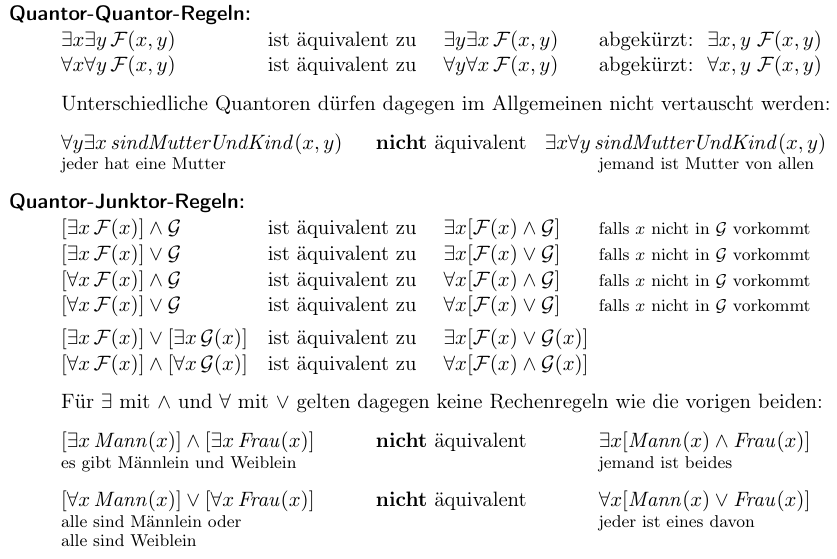
\includegraphics[width=\textwidth]{/home/areo/Documents/Studium/Summaries/Logic/figures/Rechenregeln_fuer_Kombinationen_mit_Quantoren.png}\\ (\href[page=28]{/home/areo/Documents/Studium/Semester_5_Unterlagen/Mathematische_Logik/literature/Design_Patterns_fuer_Mathematische_Beweise_with_go_back.pdf}{reference})
                \item \alert{visualisation for combinations of quantors:}\\
                  \includegraphics[width=\textwidth]{/home/areo/Documents/Studium/Summaries/Logic/figures/visualisation_of_combinations_of_qunators.png}
              \end{itemize}
            \end{minipage}
          }
        }
      }
    }
    child {
      node {Propositional Logic / Aussagenlogik
        \resizebox{\textwidth}{!}{
          \begin{minipage}[t]{12cm}
            \begin{itemize}
              \item \href[page=230]{/home/areo/Documents/Studium/Summaries/Logic/Foundations_of_AI_all_in_one_with_go_back.pdf}{extended syntax and operator precedence} and \href[page=238]{/home/areo/Documents/Studium/Summaries/Technische_Informatik/Technische_Informatik_all_in_one_with_go_back.pdf}{syntax of boolean expressions}
              \item \alert{logic formula:} e.g. $P \vee Q$, \alert{atomic formula / atomic proposition / atom:} e.g. $P$
              \begin{itemize}
                \item atomic propositions can be \alert{true} (T) or \alert{false} (F)
                \item the truth of a formula follows from the truth of its atomic propositions (\alert{truth assignment} or \alert{interpretation}) and the connectives
              \end{itemize}
            \end{itemize}
            % \begin{itemize}
            %   \item \alert{countable alphabet} of \alert{atomic propositions}: e.g. $\Sigma = \{$P, Q, R, \dots$\}$
            %   \begin{itemize}
            %     \item atomic propositions can be \alert{true} (T) or \alert{false} (F)
            %     \item the truth of a formula follows from the truth of its atomic propositions (\alert{truth assignment} or \alert{interpretation}) and the connectives.
            %   \end{itemize}
            %   \item \alert{logic formula:} e.g. $P \vee Q$, \alert{atomic formula / atom:} e.g. $P$
            %   \begin{itemize}
            %     \item \alert{operator precedence:} $\neg > \wedge > \vee > \Rightarrow > \Leftrightarrow$
            %   \end{itemize}
            %   \item \alert{literal:} (possibly negated) atomic formula
            %   \item \alert{clause:} disjunction of literals
            % \end{itemize}
          \end{minipage}
        }
      }
      child {
        node {Boolean Algebra
          \resizebox{\textwidth}{!}{
            \begin{minipage}[t]{8cm}
              \begin{itemize}
                \item \href[page=224]{/home/areo/Documents/Studium/Summaries/Technische_Informatik/Technische_Informatik_all_in_one_with_go_back.pdf}{definition, axioms}. If a sentence is directly derivable fromt the axioms, then it applies in all boolean algebras. Using properties of a concrete boolean algebra to prove a sentence is not allowed, one has to use the axioms
                \item \href[page=15]{/home/areo/Documents/Studium/Summaries/Technische_Informatik/Technische_Informatik_all_in_one_with_go_back.pdf}{conventions, precedence rulese}
                \item \href[page=231]{/home/areo/Documents/Studium/Summaries/Technische_Informatik/Technische_Informatik_all_in_one_with_go_back.pdf}{rules} derived from the axioms
              \end{itemize}
            \end{minipage}
          }
        }
        child {
          node {Boolesche Algebra der Funktionen in n Variablen $(\mathbb{B}_n, \cdot, +, \neg)$
            \resizebox{\textwidth}{!}{
              \begin{minipage}[t]{8cm}
                \begin{itemize}
                  \item \href[page=228]{/home/areo/Documents/Studium/Summaries/Technische_Informatik/Technische_Informatik_all_in_one_with_go_back.pdf}{definition}
                \end{itemize}
              \end{minipage}
            }
          }
        }
        child {
          node {Boolesche Algebra der Teilmengen von S $(Pot(S), \cap, \cup, \neg)$
            \resizebox{\textwidth}{!}{
              \begin{minipage}[t]{8cm}
                \begin{itemize}
                  \item \href[page=229]{/home/areo/Documents/Studium/Summaries/Technische_Informatik/Technische_Informatik_all_in_one_with_go_back.pdf}{definition}
                \end{itemize}
              \end{minipage}
            }
          }
        }
        child {
          node {Dualitätsprinzip bei booleschen Algebren
            \resizebox{\textwidth}{!}{
              \begin{minipage}[t]{8cm}
                \begin{itemize}
                  \item \href[page=233]{/home/areo/Documents/Studium/Summaries/Technische_Informatik/Technische_Informatik_all_in_one_with_go_back.pdf}{definition}
                \end{itemize}
              \end{minipage}
            }
          }
        }
      }
      child {
        node {Terminology
          \resizebox{\textwidth}{!}{
            \begin{minipage}[t]{12cm}
              \begin{itemize}
                \item \alert{\href[page=230]{/home/areo/Documents/Studium/Summaries/Logic/Foundations_of_AI_all_in_one_with_go_back.pdf}{literal}:} (possibly negated) atomic formula or \href[page=244]{/home/areo/Documents/Studium/Summaries/Technische_Informatik/Technische_Informatik_all_in_one_with_go_back.pdf}{alternative definition}
                \item \alert{\href[page=230]{/home/areo/Documents/Studium/Summaries/Logic/Foundations_of_AI_all_in_one_with_go_back.pdf}{clause} (germ. Klausel / \href{https://de.wikipedia.org/wiki/Disjunktionsterm}{Disjunktionsterm}):} disjunction of literals
                \item \alert{product term (germ. \href[page=245]{/home/areo/Documents/Studium/Summaries/Technische_Informatik/Technische_Informatik_all_in_one_with_go_back.pdf}{Monom} / \href{https://de.wikipedia.org/wiki/Konjunktionsterm}{Konjunktionterm}):} Konjunktion von Literalen, in der kein Literal mehr als einmal vorkommt und zu keiner Variable sowohl das positive als auch das negative Literal vorkommt. Außerdem ist \enquote{1} ein Monom
                \begin{itemize}
                  \item \alert{minterm (germ. Minterm / vollständiges Monom / \href{https://de.wikipedia.org/wiki/Vollkonjunktion}{Vollkonjunktion}):} Monom indem jede Variable entweder als positives oder als negatives Literal vorkommt
                  \begin{itemize}
                    \item \href[page=245]{/home/areo/Documents/Studium/Summaries/Technische_Informatik/Technische_Informatik_all_in_one_with_go_back.pdf}{zu $\alpha\in \mathbb{B}^n$ gehörender Minterm} $m(\alpha)$
                  \end{itemize}
                \end{itemize}
              \end{itemize}
            \end{minipage}
          }
        }
        child {
          node {Normal Forms
            \resizebox{\textwidth}{!}{
              \begin{minipage}[t]{12cm}
                \begin{itemize}
                  \item a formula is in \alert{\href[page=238]{/home/areo/Documents/Studium/Summaries/Logic/Foundations_of_AI_all_in_one_with_go_back.pdf}{disjunctive normal form (DNF)}} if it consists of a disjunction of conjunctions of literals $l_{i,j}$:
                    \[
                      \bigvee^n_{i=1} (\bigwedge^{m_i}_{j=1} l_{i,j}) 
                    \]
                  \begin{itemize}
                    \item a formula in DNF is \alert{satisfiable} iff \alert{one disjunct} is \alert{satisfiable} (check disjunct if there's no $l\wedge \neg l$), thus checking only takes linear time
                    \item aka \alert{sum of products (SoP) (germ. \href[page=247]{/home/areo/Documents/Studium/Summaries/Technische_Informatik/Technische_Informatik_all_in_one_with_go_back.pdf}{Polynom}):} Disjunktion von paarweise verschiedenen Monomen. Außerdem ist „0” ein Polynom. Ein Polynom für f heißt auch disjunktive Normalform (DNF) von f
                    \item \alert{canonical disjunctive normal form (CDNF) (germ. vollständiges Polynom):} Polynom indem alle Monome des Polynoms vollständig sind. Ein vollständiges Polynom für f heißt auch \alert{\href[page=248]{/home/areo/Documents/Studium/Summaries/Technische_Informatik/Technische_Informatik_all_in_one_with_go_back.pdf}{kanonische disjunktive Normalform (KDNF)}} von f
                  \end{itemize}
                  \item a formula is in \alert{conjunctive normal form (CNF)} if it consists of a conjunction of disjunctions of literals $l_{i,j}$:
                    \[
                      \bigwedge^n_{i=1} (\bigvee^{m_i}_{j=1} l_{i,j}) 
                    \]
                  \begin{itemize}
                    \item a formula in CNF is \alert{valid} iff \alert{every conjunct} is \alert{valid} (check conjunct if there's a $l\vee \neg l$), thus checking only takes linear time
                    \item aka \alert{product of sums (PoS)}
                    \item \alert{canonical conjunctive normal form (CCNF)} does also exist like the CDNF for the DNF
                  \end{itemize}
                  \item for every formula, there exists at least one equivalent formula in CNF and one in DNF
                  \item \href[page=239]{/home/areo/Documents/Studium/Summaries/Logic/Foundations_of_AI_all_in_one_with_go_back.pdf}{Algorithm to produce CNF or DNF}
                  \item \href[page=238]{/home/areo/Documents/Studium/Summaries/Logic/Foundations_of_AI_all_in_one_with_go_back.pdf}{reference}
                \end{itemize}
              \end{minipage}
            }
          }
        }
      }
      % child {
      %   node {Syntax and Semantics
      %     \resizebox{\textwidth}{!}{
      %       \begin{minipage}[t]{12cm}
      %         \begin{itemize}
      %           \item \alert{Sentences} are expressed according to the syntax of the representation language
      %           \begin{itemize}
      %             \item \alert{Syntax} specifies all the sentences that are well-formed
      %             \begin{itemize}
      %               \item $x + y = 4$ is a well-formed sentence
      %               \item $x4y+ =$ is not a well-formed sentence
      %             \end{itemize}
      %             \item A logic also defines the \alert{semantics} (meaning) of sentences
      %             \begin{itemize}
      %               \item Defines the \alert{truth} of a sentence with respect to each possible world
      %               \item E.g., specifies that the sentence $x + y = 4$ is true in a world in which $x = 2$ and $y = 2$, but not in a world in which $x = 1$ and $y = 1$
      %             \end{itemize}
      %           \end{itemize}
      %         \end{itemize}
      %       \end{minipage}
      %     }
      %   }
      % }
      child {
        node {Logical Entailment / Logische Ableitung bzw. Deduktion
          \resizebox{\textwidth}{!}{
            \begin{minipage}[t]{12cm}
              \begin{itemize}
                \item $\alpha \models \beta$ \alert{if} $M(\alpha) \subseteq M(\beta)$ \alert{iff} in every model in which $\alpha$ is true, $\beta$ is also true
                \begin{itemize}
                  \item $\approx $ \href[page=269]{/home/areo/Documents/Studium/Summaries/Technische_Informatik/Technische_Informatik_all_in_one_with_go_back.pdf}{less equal} for boolean functions $f, g\in\mathbb{B}_n$: $f\le g$ \alert{if} $\forall\alpha\in\mathbb{B}^n: f(\alpha)\le g(\alpha)$ \alert{iff} $ON(f)\subseteq ON(g)$
                  \item when a sentence $\beta$ \alert{\enquote{logically follows}} from another sentence $\alpha$, $\alpha$ \alert{\enquote{entails}} $\beta$
                  \item \href[page=224]{/home/areo/Documents/Studium/Summaries/Logic/Foundations_of_AI_all_in_one_with_go_back.pdf}{reference 1} and \href[page=226]{/home/areo/Documents/Studium/Summaries/Logic/Foundations_of_AI_all_in_one_with_go_back.pdf}{reference 2}
                \end{itemize}
                  \item the formula $\varphi$ \alert{follows logically} from a theory if $\varphi$ is true in all models of the theory (symbolically $theory \models \varphi$): $theory \models \varphi$ \alert{iff} $I \models \varphi$ for all models $I$ of $theory$
                  \begin{itemize}
                    \item \href[page=241]{/home/areo/Documents/Studium/Summaries/Logic/Foundations_of_AI_all_in_one_with_go_back.pdf}{reference}
                  \end{itemize}
                  \item $I \models \varphi$: Interpretation $I$ \alert{\enquote{satisfies}} a formula $\varphi$ or $\varphi$ \alert{\enquote{is true under}} $I$ when $I(\varphi) = T$
                  \begin{itemize}
                    \item an interpretation is a model of a \alert{theory} if it satisfies all formulae of the set
                    \item a formula $\varphi$ is
                    \begin{itemize}
                      \item \alert{satisfiable} if there exists $I$ that satisfies $\varphi$
                      \item \alert{unsatisfiable} if $\varphi$ is not satisfiable
                      \item \alert{falsifiable} if there exists $I$ that doesn't satisfy $\varphi$
                      \item \alert{valid} (a \alert{tautology}) if $I\models \varphi$ holds for all $I$
                    \end{itemize}
                    \item two formulae are
                    \begin{itemize}
                      \item \alert{logically equivalent} ($\varphi \equiv \psi$) if $I\models \varphi$ \alert{iff} $I\models \psi$ holds for all $I$
                    \end{itemize}
                    \item \href[page=235]{/home/areo/Documents/Studium/Summaries/Logic/Foundations_of_AI_all_in_one_with_go_back.pdf}{reference}
                  \end{itemize}
                  \item the \enquote{$\models$} symbol is a meta symbol, a meta version of \enquote{$\Rightarrow$}
                  \begin{itemize}
                    \item \alert{semantic relation} between models of a theory or a single sentence and models of a sentence
                  \end{itemize}
              \end{itemize}
            \end{minipage}
          }
        }
          child {
            node (models) {Models
              \resizebox{\textwidth}{!}{
                \begin{minipage}[t]{8cm}
                  \begin{itemize}
                    \item if a sentence $\alpha$ is true in a possible \alert{world} $m$, we say that $m$ \alert{satisfies} $\alpha$ or $m$ is a \alert{model} of $\alpha$
                    \begin{itemize}
                      \item We denote the set of all models of $\alpha$ by $M(\alpha)$ ($\hat=$ \href[page=249]{/home/areo/Documents/Studium/Summaries/Technische_Informatik/Technische_Informatik_all_in_one_with_go_back.pdf}{On-Menge})
                    \end{itemize}
                    \item an \alert{interpretation} $I$ is called a model of $\varphi$ if $I\models \varphi$
                  \end{itemize}
                \end{minipage}
              }
            }
          }
          child {
            node {Theory
              \resizebox{\textwidth}{!}{
                \begin{minipage}[t]{8cm}
                  \begin{itemize}
                    \item a \alert{set of sentences} in a formal language
                  \end{itemize}
                \end{minipage}
              }
            }
          }
          child {
            node {Interpretation
              \resizebox{\textwidth}{!}{
                \begin{minipage}[t]{8cm}
                  \begin{itemize}
                    \item \alert{truth assignment} of the atoms in $\Sigma$, corresponds to \alert{semantics} (\href[page=237]{/home/areo/Documents/Studium/Summaries/Technische_Informatik/Technische_Informatik_all_in_one_with_go_back.pdf}{reference})
                    \item $I: \Sigma \mapsto \{T, F\}$
                    \item \href[page=232]{/home/areo/Documents/Studium/Summaries/Logic/Foundations_of_AI_all_in_one_with_go_back.pdf}{extended inductive definition} and \href[page=240]{/home/areo/Documents/Studium/Summaries/Technische_Informatik/Technische_Informatik_all_in_one_with_go_back.pdf}{inductive definition with regard to boolean expressions} of the interpretation function
                  \end{itemize}
                \end{minipage}
              }
            }
          }
          child {
            node {Inference
              \resizebox{\textwidth}{!}{
                \begin{minipage}[t]{8cm}
                  \begin{itemize}
                    \item $theory \vdash_i \alpha$: generate / derive a sentence $\alpha$ with an inference method $i$
                    \item like to have inference algorithms that derive only sentences that are entailed (\alert{soundness}) and all of them (\alert{completeness})
                    \item \href[page=226]{/home/areo/Documents/Studium/Summaries/Logic/Foundations_of_AI_all_in_one_with_go_back.pdf}{reference}
                  \end{itemize}
                \end{minipage}
              }
            }
          }
      }
    };
  \end{mindmapcontent}
  \begin{edges}
    % \edge{lo}{models} % just test
  \end{edges}
  \annotation{lo.south}{This mindmap is provided without guarantee of correctness and completeness!}
  \annotation{lo.north}{\href{/tmp/current.pdf}{go back}}
\end{mindmap}
